\documentclass{emulateapj}
\usepackage{multirow,color,wrapfig,ulem}
\usepackage {graphicx}
\usepackage{graphics}
\usepackage[dvips]{epsfig}
\newcommand{\kms}{{\ifmmode{{\mathrm{\,km\ s}^{-1}}}\else{\,km~s$^{-1}$}\fi}}
\newcommand{\lya}{{Ly-$\alpha$~}}
\begin{document}

\title{Titulo} 
\shorttitle{shorttitle}

\shortauthors{Remolina-Gutierrez, Forero-Romero \&Garavito-Camargo}

\author{ Maria Camila Remolina-Gutierrez, Jaime E. Forero-Romero, Juan N. Garavito-Camargo}
\affil{Departamento de F\'{i}sica, Universidad de los Andes, Cra. 1
No. 18A-10, Edificio Ip, Bogot\'a, Colombia}
\email{mc.remolina197@uniandes.edu.co}
\email{je.forero@uniandes.edu.co}
\email{jn.garavito57@uniandes.edu.co}

\keywords{Lyman Alpha Emission,  } 
\begin{abstract}
Here goes the abstract....
\end{abstract}

\section{Introduction}
\label{sec:intro}

The Lyman-Alpha emission line is the spectral line produced when an electron goes from the second energy level to the first, loosing energy and emmiting it as light. When this energy decays are seen in Hydrogen atoms, the wavelenght of the \lya line is 121.567 nm. The detection of this emission line is a main tecnique in extragalactic astronomy because galaxies with a strong emission of this (called Lyman Alpha Emitters - LAEs) are used to study the evolution of the universe in big scale. \\

LAEs are young and far away galaxies with most of its matter composed by Hydrogen atoms, being the rest heavier elements, like Iron, produced by growing stars burning their material. Then, this spectral line tells very important information about the galaxy, most of it actually, which creates a motivation to find a way to model the \lya line according to certain free parameters that vary from a galaxy to another and that can be obtained from observations. \\

Our purpose in this paper is then to make a theoretical model, based on radiative transfer simulations, that use MonteCarlo computational methods to emulate how the line profile is going to come out of the galaxy if it is rotating and has a surrounding outflow, both of this phenomena characterized by key parameters that are going to be described further on the paper. \\

---------------------------------------------------------------------\\
MISSING: What has been done related to this? (In the astronomy world)\\
-----------------------------------------------------------------------\\

---------------------------------------------------------------------\\
MISSING: Intro to rotation model (and its analytic aproximation)\\
-----------------------------------------------------------------------\\

---------------------------------------------------------------------\\
MISSING: Intro to the ThinShell outflow model\\
-----------------------------------------------------------------------\\


\section{Theoretical Frame}
In this section we are going to describes the two different models that are used in this project, that are able to reproduce a real and consistent line.\\

---------------------------------------------------------------------\\
MISSING: \\
- Express prettier the intro of the section\\
-----------------------------------------------------------------------\\


\subsection{Rotation Model}

---------------------------------------------------------------------\\
MISSING: \\
- Full explanation.\\
- Ref: Jaime And Juan Nicolas\\
-----------------------------------------------------------------------\\


\subsection{Outflow Model: ThinShell}

---------------------------------------------------------------------\\
MISSING:\\
- Important equations and description of the parameters\\
- Why we use ThinShel instead of Wind. Its advantages (explains redshift, avoids re-difussion, bounces).\\
- Ref: Alvaro and Julian
-----------------------------------------------------------------------\\

\subsection{Joint Model}

---------------------------------------------------------------------\\
MISSING: \\
- Full explanation.\\
- How exactly are this 2 mixed\\
- Tell and make a detailed explanation of the free parameters that we are going to explore. \\
-----------------------------------------------------------------------\\

\section{Results}
\label{sec:results}
Here goes the results....

---------------------------------------------------------------------\\
MISSING: \\
- What are the compact results.\\
- Some plots.\\
- Not a physical analysis yet. \\
-----------------------------------------------------------------------\\

\section{Discussion}
\label{sec:discussion}

---------------------------------------------------------------------\\
MISSING: \\
- Comparison with some other result (probably observations).\\
- Why is this result useful? \\
- What possible implications can this model have?\\
-----------------------------------------------------------------------\\

\section{Conclusions}
\label{sec:conclusions}
Here goes the conclusions....

\section*{Acknowledgments}

To 

The data, source code and instructions to
replicate the results of this paper can be found
here {\texttt{https://github.com/mariacamilaremolinagutierrez/ LymanAlpha/}}.
Most of our code benefits from the work of the IPython and Matplotlib
communities \citep{IPython,matplotlib}.

---------------------------------------------------------------------\\
MISSING: \\
- Help from Alvaro and Julian: data, explanations, advice and collaboration. \\
- Soooo many more acknowledgments.\\
-----------------------------------------------------------------------\\

---------------------------------------------------------------------\\
MISSING IN REFERENCES: \\
- A loooot of references not here yet.\\
- Alvaro's paper.(Can galactic outflows explain the properties of Lyα emitters?
Alvaro Orsi, Cedric G. Lacey and Carlton M. Baugh)\\
- Use the correct citation method. \\
-----------------------------------------------------------------------\\

\bibliographystyle{apj}
\begin{thebibliography}{38}
\expandafter\ifx\csname natexlab\endcsname\relax\def\natexlab#1{#1}\fi

\bibitem[{{Forero-Romero} {et~al.}(2011){Forero-Romero}, {Yepes},
  {Gottl{\"o}ber}, {Knollmann}, {Cuesta}, \& {Prada}}]{CLARA}
{Forero-Romero}, J.~E., {Yepes}, G., {Gottl{\"o}ber}, S., {Knollmann}, S.~R.,
  {Cuesta}, A.~J., \& {Prada}, F. 2011, \mnras, 415, 3666
  
\bibitem[{{Verhamme} {et~al.}(2006){Verhamme}, {Schaerer}, \&
  {Maselli}}]{Verhamme06}
{Verhamme}, A., {Schaerer}, D., \& {Maselli}, A. 2006, \aap, 460, 397

\bibitem[{P\'erez \& Granger(2007)}]{IPython}
P\'erez, F., \& Granger, B.~E. 2007, Computing in Science and Engineering, 9, 21

\end{thebibliography}

\newpage

%\section{Ejemplos para tener en cuenta}
%\label{sec:implementation}
%
%Ejemplo de ecuacion
%  
%\begin{equation}
%    v_{x}=-\frac{y}{R}V_{\rm max}, \label{subeq1}
%\end{equation}
%
%Ejemplo referencia a figura
%
%In Fig. \ref{fig:geometry} se ve .....
%
%Ejemplo cita 
%
%Scape of  at line center, which has also been associated with escape of ionizing (LyC) photons
%\citep{Behrens2014,2014arXiv1404.2958V}
% 
%Ejemplo display math
%
%\begin{displaymath}
%J(x,b,\phi,i)=\frac{\sqrt{\pi}}{\sqrt{24}a\tau_0}\Bigg{(}\frac{(x-x_{\rm
%    b})^2}{1+{\rm cosh}\Big{[}\sqrt{\frac{2\pi^3}{27}}\frac{|(x
%      -x_{\rm b})^3|}{a\tau_0}\Big{]}}\Bigg{)},
%\end{displaymath} 
%
%Ejemplo de figura
%
%\begin{figure}
%\begin{center}
%  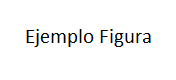
\includegraphics[width=0.4\textwidth]{ejemplofigura}
%\end{center}
%\caption{Ejemplo caption figura.  
%    \label{fig:geometry}}  
%\end{figure}
%
%Ejemplo tabla
%
%\begin{table}
%\begin{center}
%\begin{tabular}{c cccccc}
%\hline \hline
%Source & $\tau_{H}$ & &  $\ V_{\rm max}$& & \\
%Distribution& &    & (\kms) & & \\ 
%& & 0 & 100 &200 & 300\\ \hline 
%Homogeneous & $10^{5}$& 0.263 &  0.263 &  0.263 &  0.263  \\
%            & $10^{6}$ & 0.291 &   0.292 &  0.293 &  0.293 \\
%Central & $10^{5}$ &  0.096 & 0.096 &  0.096 & 0.096 \\
%  		&$10^{6}$ & 0.066 &  0.066 &  0.066 &  0.066 \\
%\hline
%\end{tabular}
%\caption{
% Ejemplo de tabla. } 
%\label{table:escape}
%\end{center}
%\end{table}

\end{document}